\section{Mu2e computing organization}
\label{sec:mu2eorg}

Mu2e is organized into two major divisions under the direct supervision of the experiment leadership: operations and analysis. Computing is distributed across these two groups. Offline computing is the responsibility of Analysis, while Online computing is part of Operations. The trigger software overlaps both sides; real-time issues are managed by the Operations group, but the algorithmic content and physics selections made by the trigger are managed by the Analysis group. The event processing framework (art), conditions data infrastructure, event display, and some data monitoring tools are also shared between Online and Offline. The formal transition between Online and Offline data processing occurs once raw data art files have been written to the data logging disk buffers by the DAQ system. 

\begin{figure}[htb]
\begin{center}
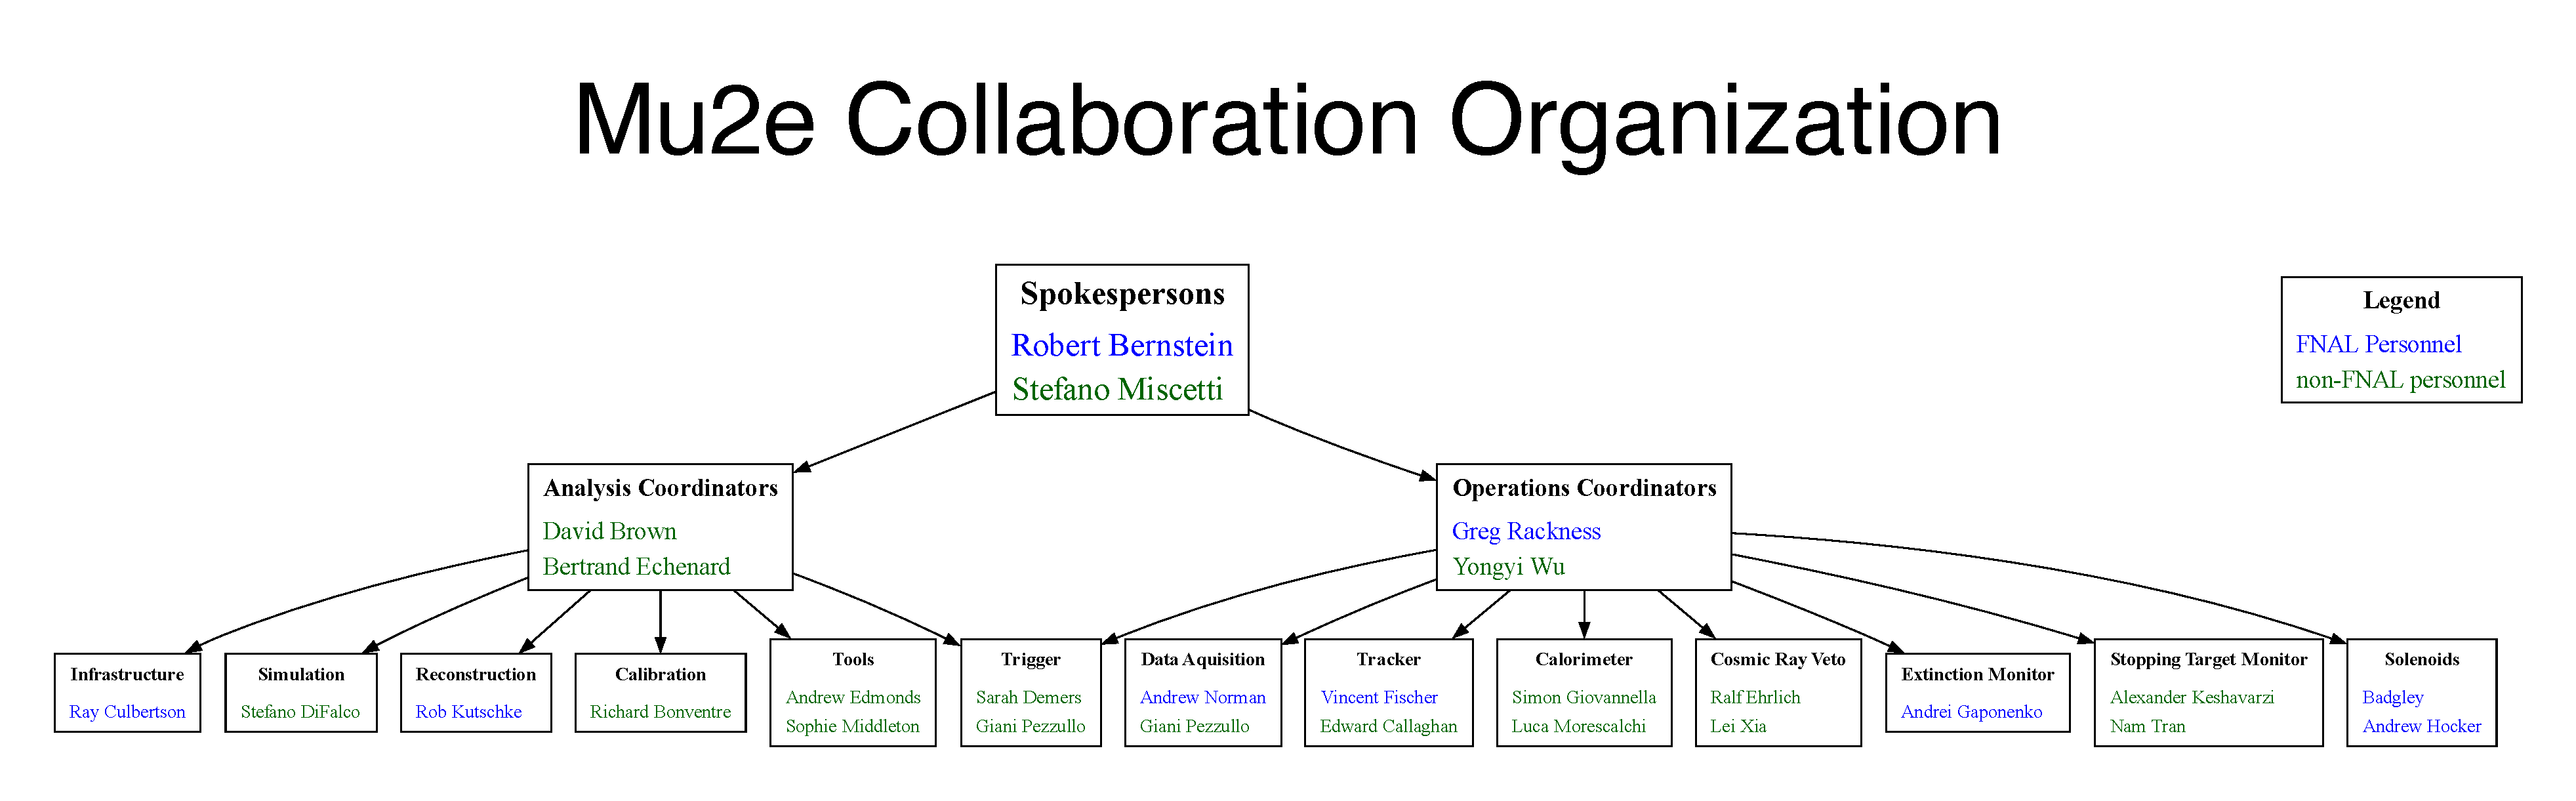
\includegraphics[width=0.95\linewidth]{figures/OrgChart_L3.pdf}
\caption{Mu2e experiment collaboration chart, June 2024.}
\label{fig:orgchartMu2e}
\end{center}
\end{figure}

\begin{figure}[htb]
\begin{center}
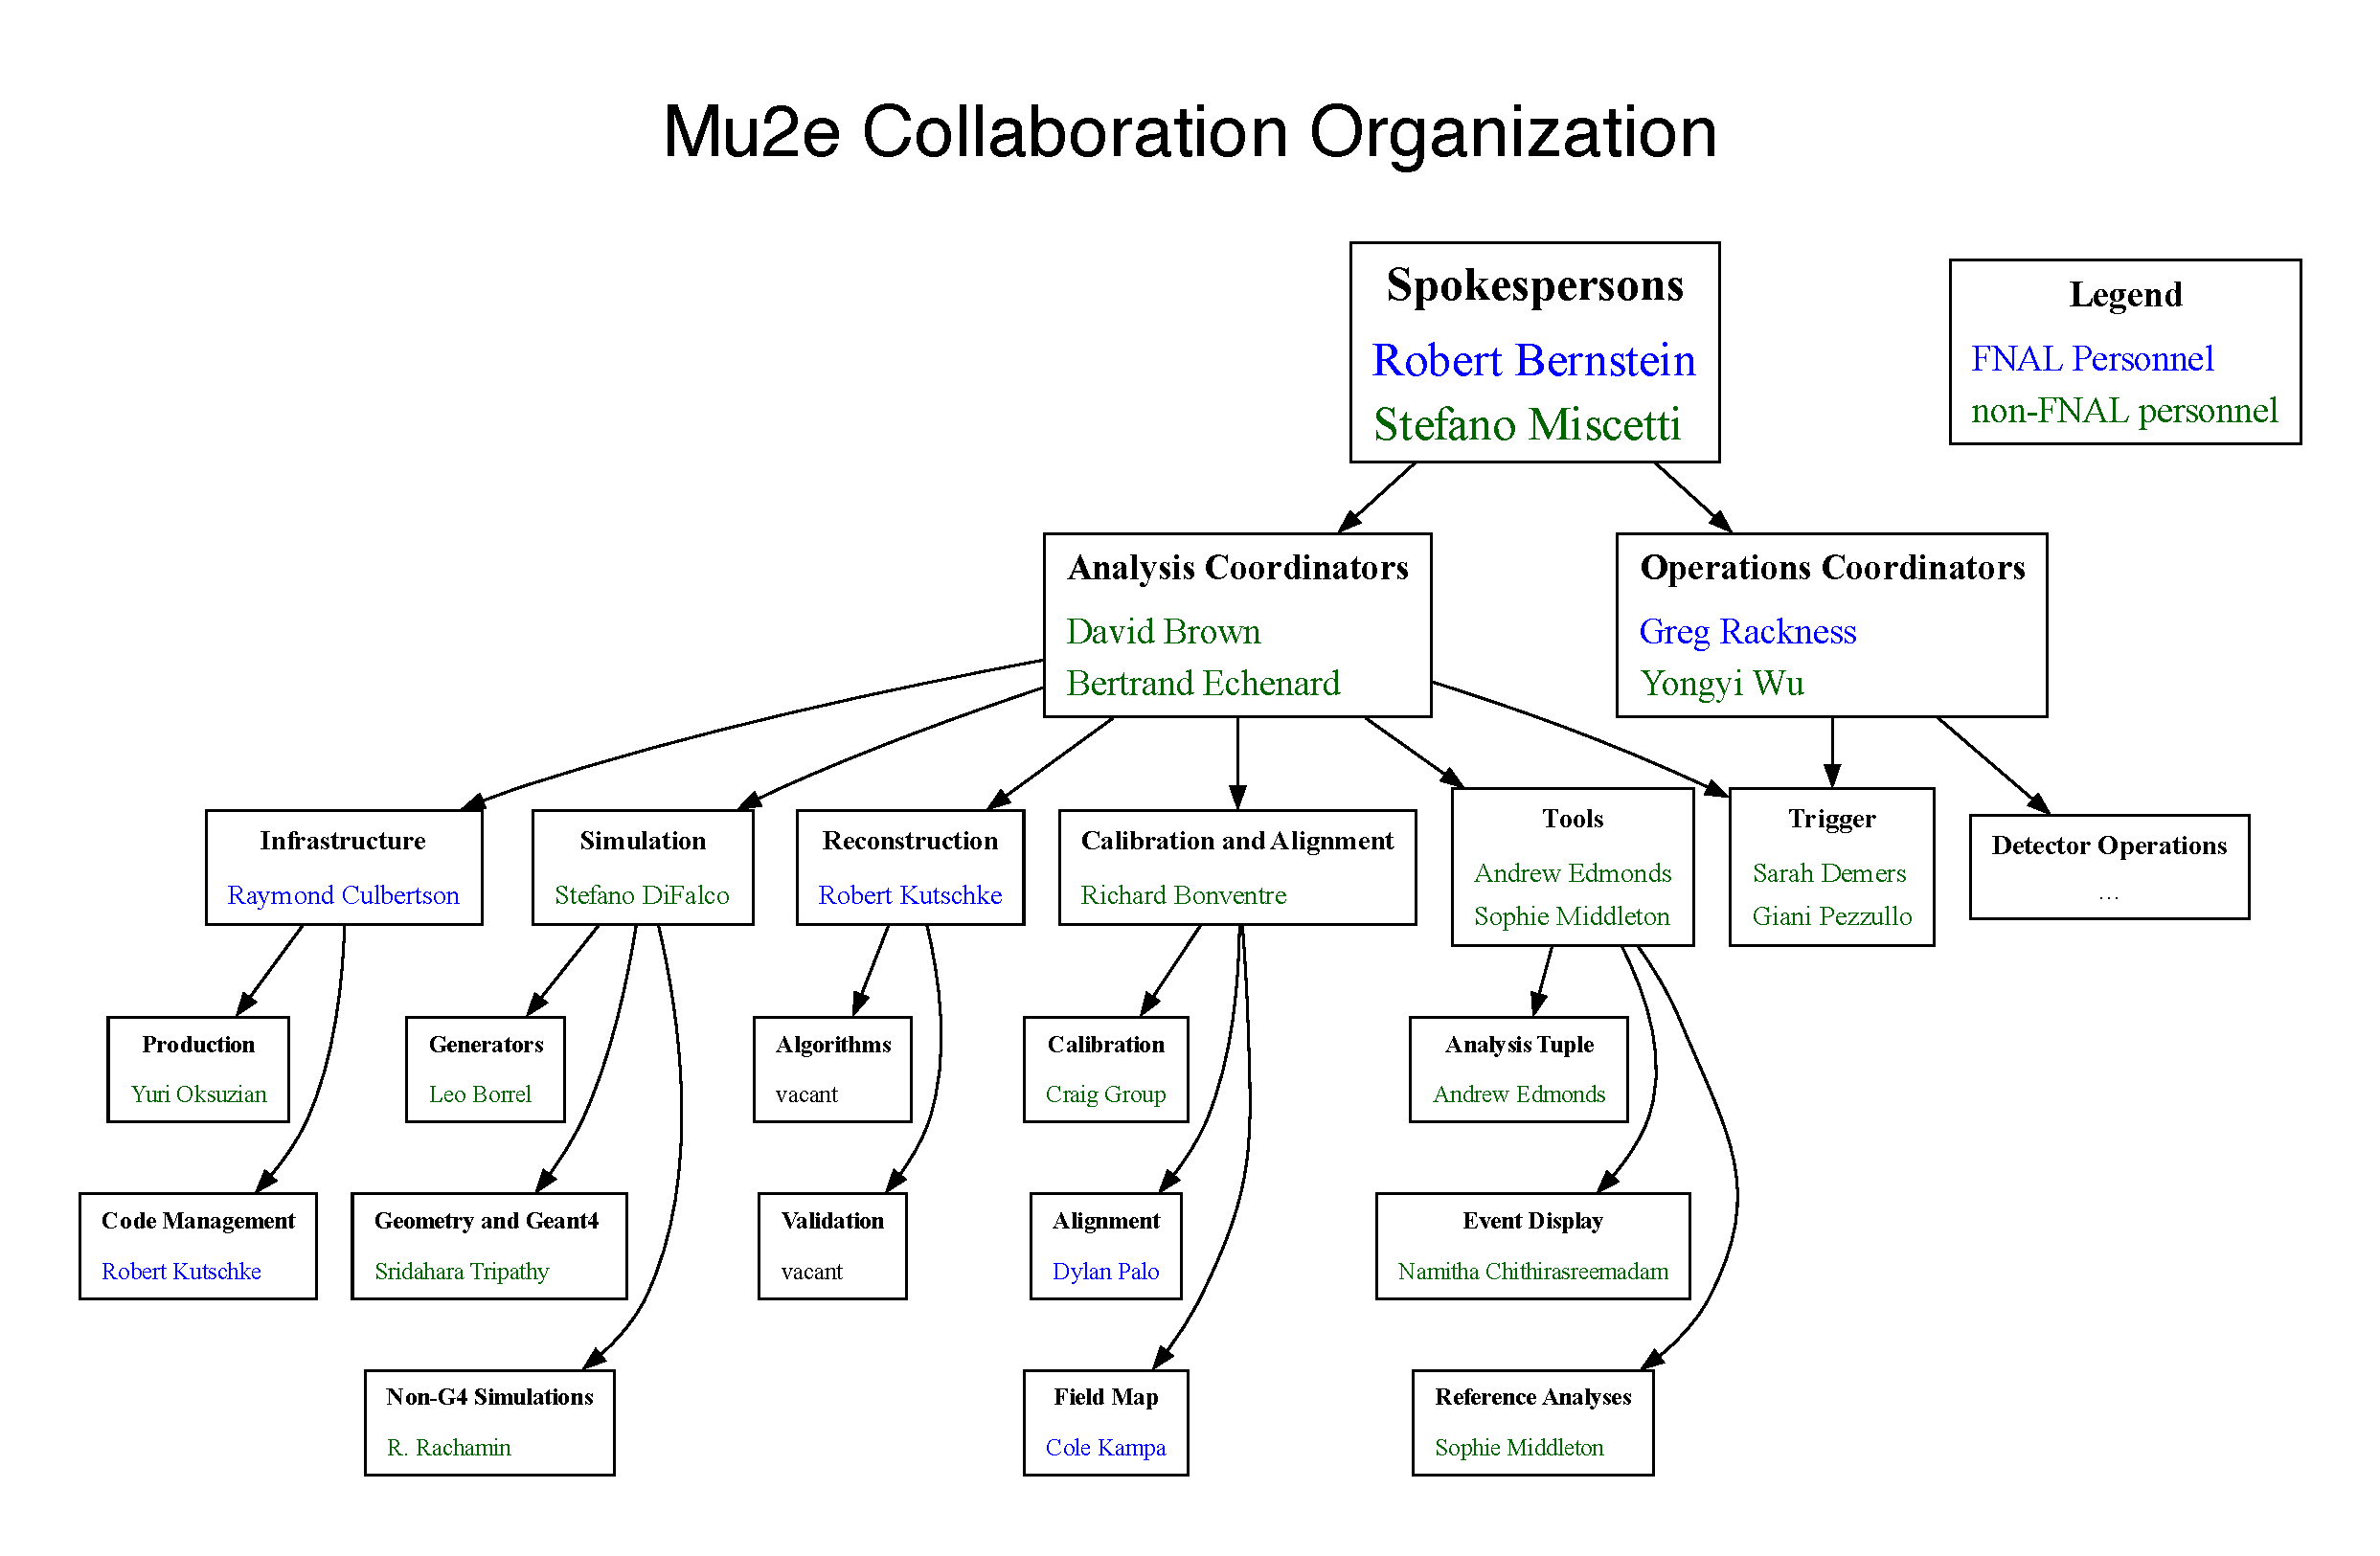
\includegraphics[width=0.95\linewidth]{figures/OrgChart_Analysis.pdf}
\caption{Mu2e Analysis Organization as of June 2024.}
\label{fig:orgchart}
\end{center}
\end{figure}



\subsection{Internal organization}
The Mu2e organization chart is shown in Figure~\ref{fig:orgchart}. Under the Analysis branch, Offline computing is divided among several Core Groups responsible for providing tools and expertise for the collaboration, ensuring experiment-wide coherence, and minimizing duplication of effort. The five core groups, and a summary of their charges from \cite{corecharge}, are given below:

\begin{itemize}

\item[] {\bf calibration \& alignment} - supervises the development of Offline tools and procedures to align and calibrate the various Mu2e detector systems and coordinate the data processing required to derive calibration and alignment values. This group is also responsible for estimating the statistical and systematic uncertainties on the alignment and calibration parameters, integrating constraints on the overall momentum scale coming from dedicated measurements, determining the calibration and alignment parameters used in simulation, and defining the quantities required to monitor the detector response and validate the agreement of detector simulations with the data.

\item[] {\bf simulation} - develops and validates the Monte Carlo generators used to model signal and background components relevant to Mu2e analyses, based on the best available theoretical models and experimental data. This group is also responsible for maintaining the description of the detector geometry and materials in the simulation, and developing Mu2e detector simulations in different Monte Carlo frameworks (e.g. FLUKA) to establish systematic uncertainties inherent to the Geant4 simulation.

\item[] {\bf reconstruction} - develops and characterizes the high-level algorithms used to create physics objects (e.,g. background hit removal, track reconstruction, or calorimeter clustering) used in calibration, analysis, and trigger selections. This group also ensures that the reconstruction algorithms used in the trigger meet DAQ requirements, and it defines the reconstruction outputs to be monitored in the validation and Continuous Integration (CI) systems. 

\item[] {\bf infrastructure and production} - manages the offline computing infrastructure and hardware resources to ensure event data, simulated event data, and conditions data are delivered for analysis in a timely and accessible way. This group maintains tools to perform data transfer between the online DAQ storage and offline storage, build and distribute the Mu2e software, access data sets catalogs, access and export Mu2e data offsite, maintain offline conditions databases, and perform offline data quality monitoring and continuous integration testing of the Mu2e Offline code base. It is also responsible for collaborating with CSAID and other resource providers to ensure access to the computational resources and technical expertise required by Mu2e.

\item[] {\bf analysis tools} - develops the tools required to perform the various physics analyses within the collaboration, including the definition of an analysis framework for the experiment with reduced data formats (aka ntuples), event display(s), and reference analyses to evaluate the impact of reconstruction code developments on the experimental sensitivity.

\end{itemize}

Additional responsibilities are shared by all groups, such as documenting tools and procedures, or ensuring that the codes meet Mu2e coding standards and performance requirements. A complete description of the core groups is available in Ref.~\cite{docdb48639}. 

Interfaces between Offline computing and the Mu2e experiment are managed at several levels. Offline computing is represented by the Analysis coordinators during weekly meetings with the experiment leadership and Operation coordinators. The analysis coordinators (or their designees)  also attend relevant meetings, including DAQ, online computing, and operation coordination. In addition, core group conveners are meeting regularly to discuss issues pertaining to Offline computing. Finally, working groups within each core group are in contact with detector and DAQ experts to coordinate computing and software development.


